\section{Scheduling and Partial Orders}

\frame{
{Part 3: Scheduling and Partial Orders}

\tableofcontents[currentsection,hideallsubsections, firstsection=1, sections={1-3}]
}

\subsection{Scheduling}

\begin{frame}
  \frametitle{Using DAGs for Scheduling}

  Let's consider again using DAGs for calculating course prerequisites.\medskip

  \begin{columns}[T]
    \column{0.3\textwidth}
    $18.01 \rightarrow 6.042$\\
    $18.01 \rightarrow 18.02$\\
    $18.01 \rightarrow 18.03$
    \column{0.35\textwidth}
    $6.001 \rightarrow 6.034$\\
    $6.042 \rightarrow 6.046$\\
    $8.02 \rightarrow 6.002$\\
    $18.03, 6.002 \rightarrow 6.004$
    \column{0.35\textwidth}
    $6.001, 6.004 \rightarrow 6.033$\\
    $6.033 \rightarrow 6.857$\\
    $6.046 \rightarrow 6.840$
  \end{columns}

  \vfill

  We say that $u$ is a \structure{indirect prerequisite} of $v$ if there is a positive length walk in graph $R$:

    \begin{center}
      $18.01 \rightarrow 6.042 \rightarrow 6.046 \rightarrow 6.840$
    \end{center}
\end{frame}



\begin{frame}{DAGs and Scheduling}{Minimal, Minimum, Maximal, Maximum of a DAG}
  \begin{columns}
    \column{0.4\textwidth}
      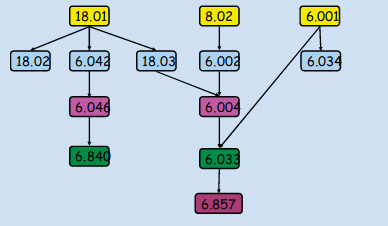
\includegraphics[width=1\textwidth]{../img/greedy_schedule}

      \column{0.6\textwidth}
    \begin{itemize}
    \item A \structure{minimal} course is does not have any prerequisites:
    \begin{itemize}
      \item $\emptyset \to 18.01$, $\emptyset \to 6.001$, $\emptyset \to  8.02$
    \end{itemize}\bigskip

    \item A \structure{minimum} course is an indirect prerequisite of {\bf all} courses.
    \begin{itemize}
      \item none in this example!
      \item if we add a course $x \to \{18.01, 8.02, 6.001\}$, then $x$ would be the minimum.
    \end{itemize}\bigskip

    \item \structure{Maximal} and \structure{maximum} courses have a similar definition.
    \begin{itemize}
      \item $\{18.02, 6.840, 6.857, 6.034\}\to \emptyset$ are maximal.
    \end{itemize}
    \end{itemize}
  \end{columns}
\end{frame}

\begin{frame}{DAG and Scheduling}{How to Schedule}

  \begin{columns}
    \column{0.4\textwidth}
      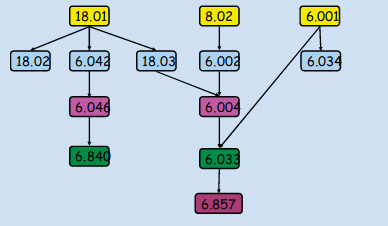
\includegraphics[width=1\textwidth]{../img/greedy_schedule}

    \column{0.6\textwidth}
      If we have the graph of course requirements, how do we select the courses for each semester? \medskip

      \structure{Greedy Scheduling}:
      \begin{enumerate}
      \item Identify Minimal Subjects;
      \item Add Minimal Subjects to Schedule;
      \item Remove Minimal Subjects;
      \item Return to Step 1
      \end{enumerate}
  \end{columns}\medskip

  Schedule:\\
  $\{18.01, 8.02, 6.001\} \to \{18.02, 6.042, 18.03, 6.002, 6.034\} \to \{6.046, 6.004\} \to \{ 6.840, 6.033\} \to 6.857$
\end{frame}


\begin{frame}{DAG and Scheduling}{Anti-Chains}
  \begin{columns}
  \column{0.4\textwidth}
    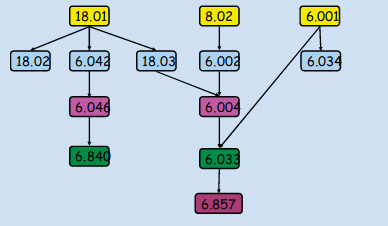
\includegraphics[width=1\textwidth]{../img/greedy_schedule}

  \column{0.6\textwidth}

    \begin{itemize}
    \item An \structure{anti-chain} is a set of vertices (courses) where there is no direct or indirect requisite relation among them.\medskip

    \item This means that the courses in an anti-chain can be taken in any order, even all at the same time.\medskip

    \item Members of an anti-chain are \structure{imcomparable}: It is not possible to say which one comes first.\medskip

    \item A relation graph can have multiple anti-chains. Example:
    \begin{itemize}
      \item $\{6.046, 6.004\}$
      \item $\{6.046, 18.03, 6.001\}$
    \end{itemize}
    \end{itemize}
  \end{columns}
\end{frame}

\begin{frame}{DAG and Scheduling}{Chains and Topological Sort}

  \begin{block}{Chains}
    Just like anti-chain is a set of vertices that have no relation among themselves, a \structure{chain} is a set of vertices that {\bf all} have a relation among themselves.
  \end{block}\medskip

  Using of chains and anti-chains, we define a \structure{Topological Sort}. A topological sort is an ordering of all vertices in $G$ that obeys the requisite relations.
  \begin{itemize}
    \item 18.01, 6.001, 8.02, 6.002, 18.03, 6.034, 6.042, 18.02, 6.004, 6.046, 6.033, 6.840, 6.857
    \item 6.001, 8.02, 6.002, 18.01, 6.034, 18.03, 18.02, 6.042, 6.004, 6.046, 6.033, 6.857, 6.840
  \end{itemize}
  If $G$ has anti-chains, it will also have multiple topological sorts.

\end{frame}

\begin{frame}{DAG and Scheduling}{Parallel Processing}

  We can use the same way of thinking to describe \structure{parallel scheduling} of tasks.\bigskip

  \begin{itemize}
    \item $n$ tasks have to be executed by $p$ processors.
    \item some pairs of tasks have a {\bf prerequisite} relation.
    \item \structure{Minimum Parallel Time}: minimum time to complete all tasks (assuming no limits on $p$)
      \begin{itemize}
        \item Minimum Parallel Time = Maximum Chain Size
      \end{itemize}
    \item \structure{Maximum Parallel Load}: value of $p$ necessary to achieve the Minimum Parallel Time
    \begin{itemize}
      \item Maximum Parallel Load $\leq$ Maximum Anti-chain Size
    \end{itemize}
  \end{itemize}
\end{frame}

\subsection{Partial Orders}

\begin{frame}[t]{Partial Orders and The Properties of a Relation}
  Until now, we observed scheduling (Partial Ordering) from the point of view of a DAG, describing the equivalent binary relation.\bigskip 

  However remember that we can go the other way to: Every binary relation can be represented as a directed graph. And if that DiGraph is also acyclic, then we can define a \structure{Partial Order} for the relation.\bigskip 
  
  So, without explicitely building the graph, how can we tell if a binary relation has a partial order?\bigskip 

  To answer that question, let's observe the properties of relations defined by DAGs.
\end{frame}

\begin{frame}[t]{Properties of Partial Orders 1: Transitivity}

  In a graph $G$, if there is a walk from $u$ to $v$, and a walk from $v$ to $w$, then there is a walk from $u$ to $w$
  \begin{center}
    \begin{tikzpicture}[scale=.5,auto,swap]
      \tikzset{edge/.style = {->,>=latex'}}
      \node[vertex] (a) at (0,0) {u};
      \node[vertex] (b) at (3,0) {v};
      \node[vertex] (c) at (6,0) {w};
      \draw[edge] (a) to (b);
      \draw[edge] (b) to (c);
      \draw[dotted] (a) to[bend right] (c);
    \end{tikzpicture}
  \end{center}\bigskip

  This defines a \structure{transitive relation}: $R(x,y)$ and $R(y,z)$ implies $R(x,y)$\bigskip 

  \emph{Lemma:} For any digraph $G$, the walk relations $G^+$ and $G^*$ are transitive.\bigskip 

  \begin{block}{Definition: Transitive Relations}
    A relation {\bf R} is transitive if:\hspace{1cm} $xRy \land yRz \implies xRz$
  \end{block}
\end{frame}

\begin{frame}[t]{Properties of Partial Orders 2: Irreflexibility}

  A binary relation $R$ from set $A$ to $A$ is \structure{reflexive} if $a~R~a$ for all $a \in A$.\bigskip 

  In the same way, a binary relation $R$ from set $A$ to $A$ is \alert{irreflexive} if NOT($a~R~a$) for all $a \in A$.\bigskip

  We have defined the 0-length walk relation $G^0$ as the directed graph where every vertex is connected to itself. Therefore, the relations $G^0$ (and $G^*$) are \structure{reflexive}.\bigskip

  On the other hand, we know that a directed graph is a DAG if it has {\bf no cycle of positive lengths}. In other words, there is no path that starts in a vertice and goes back to itself.\bigskip 

  Therefore, \alert{$R$ is a DAG iff $R^+$ is irreflexive}.\bigskip
\end{frame}

\begin{frame}[t]{Strict Partial Orders}
  With these two properties, we can define when a Relation is a \structure{Strict Partial Order}, and can be represented by A DAG:\bigskip 

  \begin{block}{}
    A binary relation is a \structure{Strict Partial Order} if it is {\bf transitive} and {\bf Irreflexive}
  \end{block}\bigskip

  Examples of strict partial orders: 
  \begin{itemize}
    \item The "Less than" relation: $a < b$
    \item The "Strict subset" relation: $A \subset B$
  \end{itemize}
\end{frame}

\begin{frame}[t]{Path Total Orders}

  A \structure{Strict Partial Order} is also \structure{Path Total} if, for any two distinct elements, one will always be ``greater than'' another.
  \bigskip

  Example: The "Less than" relation $<$ on $\mathbb{R}$ is Path Total: for any two elements $x,y \in \mathbb{R}, x \neq y$, either $x < y$ or $y < x$
  \bigskip

  Counter-Example: The "Strict subset" relation is NOT Path Total. For example, subsets $\{2, 3\}$ and $\{1, 6\}$ are incomparable, regarding subsets.\bigskip

  \begin{block}{}
  \begin{itemize}
  \item Relation $R$ is \structure{path total}: if $x \neq y \implies xRy \lor yRx$
  \item This means there are \alert{no imcomparable elements}
  \end{itemize}
  \end{block}

  In a \structure{path total} relation, the graph representing it is a 
  \structure{chain}
\begin{center}
  \begin{tikzpicture}[scale=.8,auto,swap]
    \tikzset{edge/.style = {->,>=latex'}}
    \node[vertex] (a) at (0,0) {};
    \node[vertex] (b) at (1,0) {};
    \node[vertex] (c) at (2,0) {};
    \node[vertex] (d) at (4,0) {};
    \node[vertex] (e) at (5,0) {};
    \node[vertex] (f) at (6,0) {};
    \draw[edge] (a) to (b);
    \draw[edge] (b) to (c);
    \draw[dotted] (c) to (d);
    \draw[edge] (d) to (e);
    \draw[edge] (e) to (f);
  \end{tikzpicture}
\end{center}
\end{frame}

\begin{frame}[t]{Partial Orders: Assymetry}
  
  Another way to describe a DAG is through the property of \structure{Assymetry}:\bigskip

  \begin{block}{Definition: Assymetric Relation}
    A relation {\bf R} is assymetric if: $u~R^+~v \implies \text{NOT}(v~R^+~u)$
  \end{block}\bigskip

  In other words: a relation is assymetric if a path can only exist from $u$ to $v$, or from $v$ to $u$.\bigskip 

  This makes sense, a DAG is characterized by the {\bf lack of cycles}. If there are no cycles, it is not possible to go both ways.
\end{frame}

\begin{frame}{Weak Partial Order}

  A \structure{weak partial order} is a relaxation of the \structure{strict partial order}. The difference is that each element is comparable to itself:

  \begin{center}
    \begin{tikzpicture}[scale=.8,auto,swap]
      \tikzset{edge/.style = {->,>=latex'}}
      \node[vertex] (a) at (0,0) {};
      \node[vertex] (b) at (1,0) {};
      \node[vertex] (c) at (2,0) {};
      \node[vertex] (d) at (4,0) {};
      \node[vertex] (e) at (5,0) {};
      \node[vertex] (f) at (6,0) {};
      \draw[edge] (a) to (b);
      \draw[edge] (b) to (c);
      \draw[dotted] (c) to (d);
      \draw[edge] (d) to (e);
      \draw[edge] (e) to (f);
      \draw[edge] (a) to[loop] (a);
      \draw[edge] (b) to[loop] (b);
      \draw[edge] (c) to[loop] (c);
      \draw[edge] (d) to[loop] (d);
      \draw[edge] (e) to[loop] (e);
      \draw[edge] (f) to[loop] (f);
    \end{tikzpicture}
  \end{center}\bigskip

  Examples:
  \begin{itemize}
    \item The $\leq$ relation ($1 \leq 1$)
    \item The $\subseteq$ relation ($\{1,2\} \subseteq \{1,2\}$)
  \end{itemize}\bigskip 

  Weak partial orders help us define the \alert{Antisymmetry} property:

  \begin{block}{Definition: Antissymetric Relation}
    A relation {\bf R} is antissymetric if: $u~R^+~v \implies \text{NOT}(v~R^+~u)$ ONLY WHEN $u \neq v$
  \end{block}
\end{frame}

\begin{frame}
  \frametitle{Assimetry and Antissimetry}

  {\larger

    \begin{block}{Assimetry}
      \begin{itemize}
      \item Reflexibility is \alert{never} allowed
      \item R is \structure{assimetric} {\bf iff}:
        \begin{equation*}
          xRy \implies \text{NOT}(yRx)
        \end{equation*}
      \end{itemize}

    \end{block}

    \begin{block}{Antissimetry}
      \begin{itemize}
      \item Reflexibility is allowed \alert{ONLY WHEN $x = y$}
      \item R is \structure{antissimetric} {\bf iff}
        \begin{equation*}
          xRy \implies \text{NOT}(yRx), \text{ for } x \neq y
        \end{equation*}
      \end{itemize}
    \end{block}
  }
\end{frame}


\subsection{Partial Orders and Isomorphisms}

\begin{frame}{Partial Orders and Isomorphism}{Proper Subset Relation}
  \frametitle{Proper Subset Relation}

  The proper subset relation: $A \subset B$ represents a partial order.\bigskip

  For example, the proper subset relation defined on the "recursive set of divisors of 30" is as follows:

\begin{center}
    \begin{tikzpicture}[scale=1.2,auto,swap]
      \tikzset{edge/.style = {->,>=latex'}}
      \node[vertex,label={1}] (a) at (0,1) {};
      \node[vertex,label={1,3}] (b) at (2,0) {};
      \node[vertex,label={1,5}] (c) at (2,1) {};
      \node[vertex,label={1,2}] (d) at (2,2) {};
      \node[vertex,label={1,3,5,15}] (e) at (4,0) {};
      \node[vertex,label={1,2,5,10}] (f) at (4,2) {};
      \node[vertex,label={1,2,3,5,10,15,30}] (g) at (5,1) {};
      \draw[edge] (a) to (b);
      \draw[edge] (a) to (c);
      \draw[edge] (a) to (d);
      \draw[edge] (c) to (e);
      \draw[edge] (b) to (e);
      \draw[edge] (c) to (f);
      \draw[edge] (d) to (f);
      \draw[edge] (e) to (g);
      \draw[edge] (f) to (g);
    \end{tikzpicture}
  \end{center}
\end{frame}

\begin{frame}{Partial Orders and Isomorphism}{Proper Divide Relation}

  The \structure{proper divide} relation is defined as $a R b$ if $a|b$ and $a \neq b$.\bigskip

  We can see that, for the set $\{1,2,3,5,10,15,30\}$, the proper subset relation and the proper division relation have {\bf the same relationship DAG}.\bigskip

  This means that the two relations are \structure{{\bf isomorphic}}

  \begin{center}
    \begin{tikzpicture}[scale=1.2,auto,swap]
      \tikzset{edge/.style = {->,>=latex'}}
      \node[vertex,label={1}] (a) at (0,1) {};
      \node[vertex,label={3}] (b) at (2,0) {};
      \node[vertex,label={5}] (c) at (2,1) {};
      \node[vertex,label={2}] (d) at (2,2) {};
      \node[vertex,label={15}] (e) at (4,0) {};
      \node[vertex,label={10}] (f) at (4,2) {};
      \node[vertex,label={30}] (g) at (5,1) {};
      \draw[edge] (a) to (b);
      \draw[edge] (a) to (c);
      \draw[edge] (a) to (d);
      \draw[edge] (c) to (e);
      \draw[edge] (b) to (e);
      \draw[edge] (c) to (f);
      \draw[edge] (d) to (f);
      \draw[edge] (e) to (g);
      \draw[edge] (f) to (g);
    \end{tikzpicture}
  \end{center}
\end{frame}

\begin{frame}{Isomorphism}

    \begin{itemize}
    \item Two graphs are \structure{isomorphic} if they have the same \structure{set of vertices and set of edges}\bigskip

    \item More formally, two graphs $G_1, G_2$ are \structure{isomorphic} if there is a relation $M$ which is an \emph{edge preserving maching} between their vertices.\bigskip

    \item $G_1 \text{ isomorphic } G_2 \iff \exists \text { bijection
    } M:V_1\to V_2$\\\hfill with $(u,v) \in E_1 \iff
      (M(u),M(v)) \in E_2$

    \end{itemize}
\end{frame}

%% TODO: Remember why this is important and then re-add to the lecture
% \begin{frame}
%   \frametitle{Isomorphism, $\subset$ and partial orders}
%
%   {\larger
%     {\bf Theorem:} Every strict p.o. $R$ is isomorphic to some
%     collection of sets partially ordered by $\subset$.
%
%     \bigskip
%
%     {\bf Proof (by construction):}
%     \begin{itemize}
%     \item Map element $a$ to the set of elements below it.
%     \item in other words, $a$ maps to $\{b \in A| bRa \lor b = a\}$\\
%       \hfill(remember that NOT$(aRa)$)
%     \item in other words, $f(a) ::= R^{-1}(a) \cup \{a\}$
%     \end{itemize}
%
%     \bigskip
%
%     {\bf Example:} from divides
%     \begin{itemize}
%     \item $f(10) = 1|10, 2|10, 5|10, \cup \{10\} = \{1,2,5,10\}$
%     \item $f(3) = 1|3, \cup \{3\} = \{1,3\}$
%     \end{itemize}
%   }
% \end{frame}

\subsection{Equivalence Relations}

\begin{frame}
  \frametitle{Symmetric Relations and Equivalence Relations}

  \begin{itemize}
    \item If there is a walk from $u$ to $v$ and a walk from $v$ to
      $u$, then we say that $u$ and $v$ are \structure{strongly
      connected}.
      \begin{itemize}
        \item $uG^*v$ and $vG^*u$
      \end{itemize}\bigskip

    \item The relation $R$ is \structure{symmetric} if $aRb \implies bRa$.
    \begin{itemize}
      \item The walk relation of A \structure{strongly connected} graph is symmetric.
    \end{itemize}\bigskip

    \item An \structure{equivalence relation} $R$ is: transitive,
      symmetric and reflexive.\bigskip

    \item This means that $R$ is an \structure{equivalence relation} {\bf iff} $R$ is the \structure{strongly connected} relation of some DiGraph.
    \end{itemize}
\end{frame}

\begin{frame}
  \frametitle{Equivalence Relations Examples}

  The definitions of the last slide allows us to formally define an \emph{equivalence equation}.\bigskip

  {\larger
    Examples:
    \begin{itemize}
    \item Equality: $=$
    \item $\equiv $(mod n)
    \item Same Size, Same Color, etc.
    \end{itemize}
  }\bigskip

  It may seem that an equivalence relation is too obvious to need a definition (specially for numbers!), but this can be useful when we want to define equivalence for more complex things, like sets.

\end{frame}

\begin{frame}
  \frametitle{Relation Properties: Graphical Review}

  {\larger

    \begin{columns}
      \column{0.5\textwidth}
      \begin{center}
      Reflexive:\\
      \begin{tikzpicture}[scale=1,auto,swap]
        \tikzset{edge/.style = {->,>=latex'}}
        \node[vertex] (a) at (0,0) {};
        \node[vertex] (b) at (1,0) {};
        \node[vertex] (c) at (0,1) {};
        \draw[edge] (a) to[loop] (a);
        \draw[edge] (b) to[loop](b);
        \draw[edge] (c) to[loop] (c);
        \draw[edge] (c) to (b);
      \end{tikzpicture}

      \bigskip

      Transitive:\\
      \begin{tikzpicture}[scale=1,auto,swap]
        \tikzset{edge/.style = {->,>=latex'}}
        \node[vertex] (a) at (0,0) {};
        \node[vertex] (b) at (1,0) {};
        \node[vertex] (c) at (2,0) {};
        \draw[edge] (a) to (b);
        \draw[edge] (b) to (c);
        \draw[dotted] (a) to[bend right] (c);
      \end{tikzpicture}
      \end{center}
      \column{0.5\textwidth}
      \begin{center}
      Assymetric:\\
      \begin{tikzpicture}[scale=1,auto,swap]
        \tikzset{edge/.style = {->,>=latex'}}
        \node[vertex] (a) at (0,0) {};
        \node[vertex] (b) at (1,1) {};
        \node[vertex] (c) at (2,0) {};
        \draw[edge] (a) to (b);
        \draw[edge] (b) to (c);
        \draw[edge] (a) to (c);
      \end{tikzpicture}

      \bigskip

      Symetric:\\
      \begin{tikzpicture}[scale=1,auto,swap]
        \tikzset{edge/.style = {->,>=latex'}}
        \node[vertex] (a) at (0,0) {};
        \node[vertex] (b) at (1,0) {};
        \node[vertex] (c) at (2,0) {};
        \draw[edge] (a) to[bend left] (b);
        \draw[edge] (b) to[bend left] (a);
        \draw[edge] (b) to[bend left] (c);
        \draw[edge] (c) to[bend left] (b);
      \end{tikzpicture}

      \end{center}
    \end{columns}
  }
\end{frame}


% TODO: Remember why this is important and re-introduce it!
% \begin{frame}
%   \frametitle{Representing Equivalence}
%   {\larger
%
%     \begin{itemize}
%     \item For a total function $f:A\rightarrow B$
%     \item We can define an equivalence relation: $\equiv_f$ on $A$:
%       \begin{equation}
%         a \equiv_f a' \iff f(a) = f(a')
%       \end{equation}
%
%       \bigskip
%
%     \item {\bf Theorem:} Relation $R$ on set $A$ is an equiv. relation
%       {\bf iff}: $R$ is $\equiv_f$ for some $f:A\rightarrow B$
%
%       \bigskip
%
%     \item {\bf Example:} $\equiv$ (mod n) is $\equiv_f$
%       \structure{where} $f(k) ::= \text{rem}(k,n)$
%     \end{itemize}
%   }
% \end{frame}
%
% \begin{frame}
%   \frametitle{Equivalence and Partition}
%
%   {\larger
%     \begin{itemize}
%     \item We define a \structure{partition} $\Pi$ of a set $A$, where
%       $\$Pi$ is a collection of subsets of $A$ that cover all elements
%       but do not overlap.
%
%       \bigskip
%
%       {\bf Example:} For A = $\{a,b,c,d,e\}$ one partition could be:
%       $\{a,b\},\{c,e\},\{d\}$
%
%
%       \bigskip
%
%     \item We define a relatin $\equiv_{\Pi}$ on A: $a \equiv_{\Pi} a'$
%       if both $a$ and $a'$ are in the same subset of $\Pi$
%
%       \bigskip
%
%     \item A relation $R$ on set $A$ is an equivalence relation {\bf
%       iff} $R$ is $\equiv_{\Pi}$ for some partition $\Pi$ of $A$.
%     \end{itemize}
%
%   }
% \end{frame}
